% Round 2 findings section

\subsubsection*{Round 2}
\label{sec:findings-r2}

%%%
Round 2 consisted of ten agents paired off against each other
in both the winners' and losers' brackets.
%
The winners' bracket used agents previously trained from Round 1
while the losers' bracket agents started with random initializations.
%
These agents were each trained for a million games
with mostly the same configuration as in Round 1,
except the scaling factor was lowered to $s = 2.0$
and exploration rate was set to a constant $e = 0.30$.
%%%

\paragraph*{Performance}
\label{sec:findings-r2-perf}

%%%
Judging by the lack of pattern found in
Figures~\ref{fig:r2-spreads-winner}
and~\ref{fig:r2-spreads-loser},
%and~\ref{fig:r2-spreads-random},
there is no significant performance increase to be found from Round 2.
%
If learning had occurred,
Figures~\ref{fig:r2-spreads-winner-a}
and~\ref{fig:r2-spreads-loser-a}
%and~\ref{fig:r2-spreads-random-a}
would take on the form of a decreasing curve,
gradually approaching zero,
while Figures~\ref{fig:r2-spreads-winner-b}
and~\ref{fig:r2-spreads-loser-b}
%and~\ref{fig:r2-spreads-random-b}
would be their translation across the x-axis.
%
On its own, Figure~\ref{fig:r2-spreads-winner}
would indicate that an agent trained for one million games plays on par with
one trained for two million games.
%
Alone,
this would indicate that performance had reached a peak and saturated.
%
However,
the similarity to Figure~\ref{fig:r2-spreads-loser}
%and even to Figure~\ref{fig:r2-spreads-random}
shows that neither bracket learned to perform better than previous iterations.
%%%

% Point spreads for two runs of blah

\begin{figure}
\center

\begin{subfigure}[b]{0.45\textwidth}
	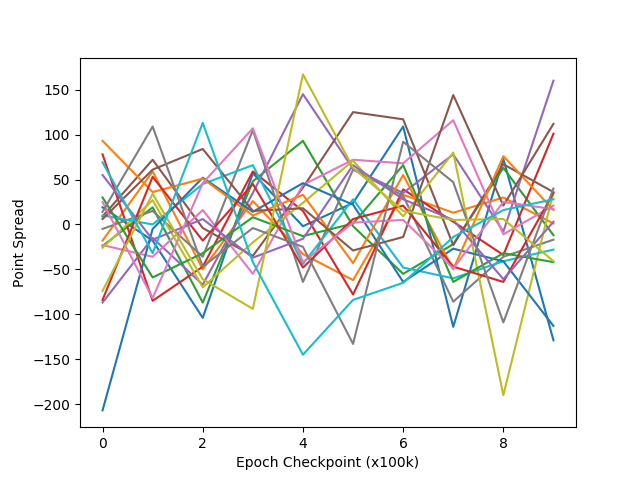
\includegraphics[width=\linewidth]{images/findings/round2/spreads_self-v-prev_winner.png}
	\caption{An agent plays against previous iterations of itself.}
	\label{fig:r2-spreads-winner-a}
\end{subfigure}
~
\begin{subfigure}[b]{0.45\textwidth}
	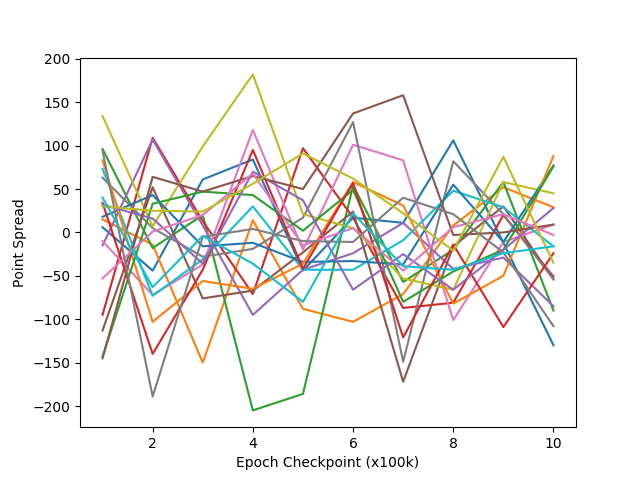
\includegraphics[width=\linewidth]{images/findings/round2/spreads_rand-v-fut_winner.png}
	\caption{A random agent plays against later, more learned agents.}
	\label{fig:r2-spreads-winner-b}
\end{subfigure}

\caption{
	Point spreads across twenty 9-game tournaments for an agent in the
	winners' bracket of Round 2.
	Note that since the winners' bracket uses an agent with prior training,
	the total epochs elapsed is one million more than displayed.
}
\label{fig:r2-spreads-winner}
\end{figure}


% Point spreads for two runs of blah

\begin{figure}
\center

\begin{subfigure}[b]{0.45\textwidth}
	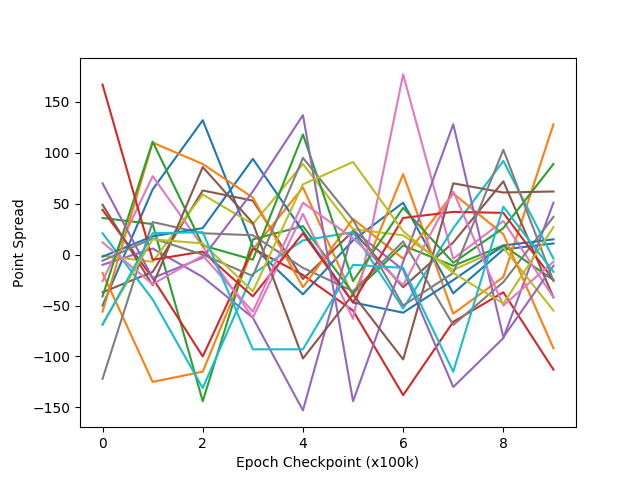
\includegraphics[width=\linewidth]{images/findings/round2/spreads_self-v-prev_loser.png}
	\caption{An agent plays against previous iterations of itself.}
	\label{fig:r2-spreads-loser-a}
\end{subfigure}
~
\begin{subfigure}[b]{0.45\textwidth}
	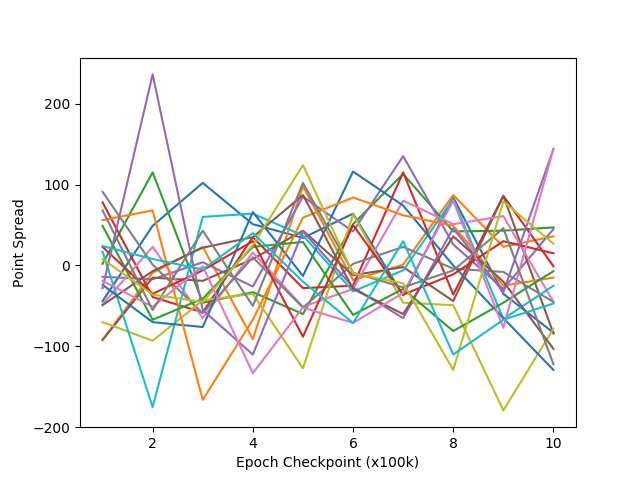
\includegraphics[width=\linewidth]{images/findings/round2/spreads_rand-v-fut_loser.png}
	\caption{A random agent plays against later, more learned agents.}
	\label{fig:r2-spreads-loser-b}
\end{subfigure}

\caption{
	Point spreads across mutliple 9-game tournamens of an agent in the
	losers' bracket of Round 2.
}
\label{fig:r2-spreads-loser}
\end{figure}


%\begin{figure}
\center

%\includegraphics[width=0.8\textwidth]{images/findings/round2/spreads_random.png}
\begin{subfigure}[b]{0.90\textwidth}
	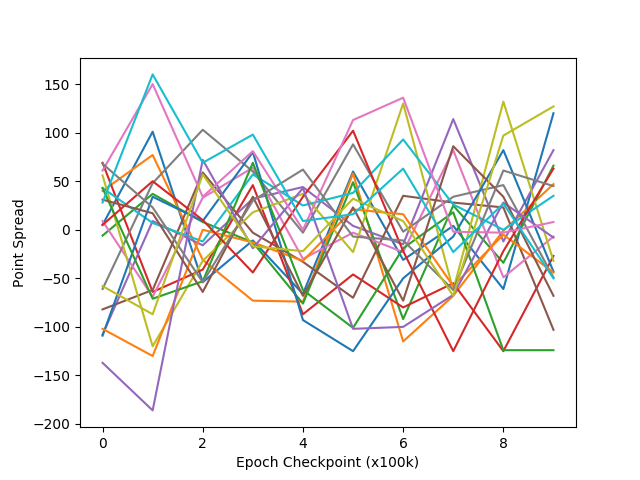
\includegraphics[width=\linewidth]{images/findings/round2/spreads_self-v-prev_random.png}
	\caption{An agent plays against previous iterations of itself.}
	\label{fig:r2-spreads-random-a}
\end{subfigure}

\begin{subfigure}[b]{0.90\textwidth}
	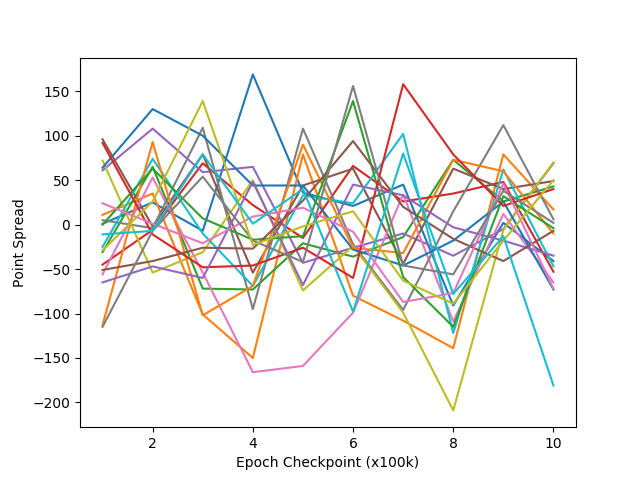
\includegraphics[width=\linewidth]{images/findings/round2/spreads_rand-v-fut_random.png}
	\caption{A random agent plays against later, more learned agents.}
	\label{fig:r2-spreads-random-b}
\end{subfigure}


\caption{
	Point spreads across mutliple 9-game tournamens of an agent
	trained against a static, unlearning agent with random weights.
}
\label{fig:r2-spreads-random}
\end{figure}




\paragraph*{Learning Process and Results}
\label{sec:findings-r2-results}

%%%
% Discussion of what it learns and why that's interesting from a cribbage
% perspective
%%%


\begin{figure}
\center

	\begin{subfigure}[t]{0.22\textwidth}
		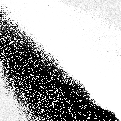
\includegraphics[width=\textwidth]{images/findings/round2/strats/winner/hand_max_min.png}
		\caption{\handmaxmin}
	\end{subfigure}
	~
	\begin{subfigure}[t]{0.22\textwidth}
		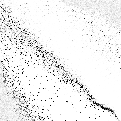
\includegraphics[width=\textwidth]{images/findings/round2/strats/winner/hand_max_avg.png}
		\caption{\handmaxavg}
	\end{subfigure}
	~
	\begin{subfigure}[t]{0.22\textwidth}
		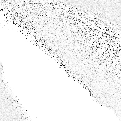
\includegraphics[width=\textwidth]{images/findings/round2/strats/winner/hand_max_med.png}
		\caption{\handmaxmed}
	\end{subfigure}
	~
	\begin{subfigure}[t]{0.22\textwidth}
		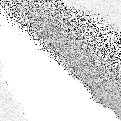
\includegraphics[width=\textwidth]{images/findings/round2/strats/winner/hand_max_poss.png}
		\caption{\handmaxposs}
	\end{subfigure}

	\begin{subfigure}[t]{0.22\textwidth}
		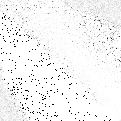
\includegraphics[width=\textwidth]{images/findings/round2/strats/winner/crib_min_avg.png}
		\caption{\cribminavg}
	\end{subfigure}
	~
	\begin{subfigure}[t]{0.22\textwidth}
		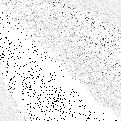
\includegraphics[width=\textwidth]{images/findings/round2/strats/winner/pegging_max_avg_gained.png}
		\caption{\peggingmaxavggained}
	\end{subfigure}
	~
	\begin{subfigure}[t]{0.22\textwidth}
		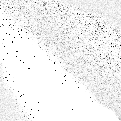
\includegraphics[width=\textwidth]{images/findings/round2/strats/winner/pegging_max_med_gained.png}
		\caption{\peggingmaxmedgained}
	\end{subfigure}
	~
	\begin{subfigure}[t]{0.22\textwidth}
		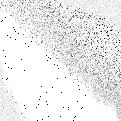
\includegraphics[width=\textwidth]{images/findings/round2/strats/winner/pegging_min_avg_given.png}
		\caption{\peggingminavggiven}
	\end{subfigure}

\caption{
	All final strategy strengths for an agent in the winners' bracket
	when playing as the dealer
	after training for one million games during Round 1
	and a further one million games during Round 2.
}
\label{fig:r2-strats-winner}
\end{figure}


%%%
Despite the lack of performance increase after another million games played by
both the winners' and losers' brackets,
there are still interesting trends to be spotted between the different brackets
of play.
%
The most notable is how quickly policies converge to a similar state.
%
While the strategy graphs for the less trained agents are less crisp
in their appearance thanks to their slower learning rates,
the patterns of which policy to mainly follow at which times
are still quick to form.
%%%

%%%
Even more fascinating observations can be found from the strategy graphs
from the winners' bracket (see Figure~\ref{fig:r2-strats-winner}).
%
By focusing on the \handmaxmin\ and \handmaxavg\ strategies in particular,
the sinusoidal wave along the diagonal can be observed extending further
back along the diagonal to earlier game positions,
albeit with smaller amplitude.
%
While not being of much use to the agent directly,
this is a useful observation from a cribbage player's perspective.
%
Since it is possible to infer the state-value function,
the implications of this wave are that earlier states are not crucial
predictors for future success.
%
Not only that,
but the agent has learned that changes in lead are likely in later game states
and not necessarily detrimental to the ability to win the game.
%%%

%%%%
%Care needs to be taken with this previous observation on the wave's amplitude
%and it must be pointed out to be speculation on the part of the author.
%%
%It may be the case that with enough training the sine wave will be at full
%amplitude in earlier positions.
%%
%A reminder must be made that
%a notable reason for the lack of clarity at the moment is the weight adjustment
%mechanism for training.
%%
%The training system pre-supposes that the earlier positions are of less
%importance in a game and adjusts them with a lower priority than later positions
%in the game.
%%
%It may indeed be the case that two million games is still not enough to
%counteract the decay of temporal difference learning with the learning
%rate used.
%%%%


%%%
% Talking about losers' bracket and how it compares to winner's
%%%


\begin{figure}
\center

	\begin{subfigure}[t]{0.22\textwidth}
		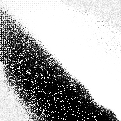
\includegraphics[width=\stratgraphwidth]{images/findings/round2/strats/loser/hand_max_min.png}
		\caption{\handmaxmin}
	\end{subfigure}
	~
	\begin{subfigure}[t]{0.22\textwidth}
		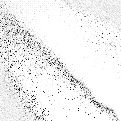
\includegraphics[width=\stratgraphwidth]{images/findings/round2/strats/loser/hand_max_avg.png}
		\caption{\handmaxavg}
	\end{subfigure}
	~
	\begin{subfigure}[t]{0.22\textwidth}
		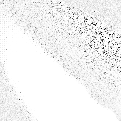
\includegraphics[width=\stratgraphwidth]{images/findings/round2/strats/loser/hand_max_med.png}
		\caption{\handmaxmed}
	\end{subfigure}
	~
	\begin{subfigure}[t]{0.22\textwidth}
		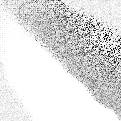
\includegraphics[width=\stratgraphwidth]{images/findings/round2/strats/loser/hand_max_poss.png}
		\caption{\handmaxposs}
	\end{subfigure}

	\begin{subfigure}[t]{0.22\textwidth}
		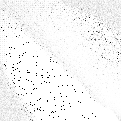
\includegraphics[width=\stratgraphwidth]{images/findings/round2/strats/loser/crib_min_avg.png}
		\caption{\cribminavg}
	\end{subfigure}
	~
	\begin{subfigure}[t]{0.22\textwidth}
		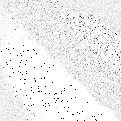
\includegraphics[width=\stratgraphwidth]{images/findings/round2/strats/loser/pegging_max_avg_gained.png}
		\caption{\peggingmaxavggained}
	\end{subfigure}
	~
	\begin{subfigure}[t]{0.22\textwidth}
		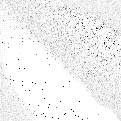
\includegraphics[width=\stratgraphwidth]{images/findings/round2/strats/loser/pegging_max_med_gained.png}
		\caption{\peggingmaxmedgained}
	\end{subfigure}
	~
	\begin{subfigure}[t]{0.22\textwidth}
		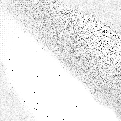
\includegraphics[width=\stratgraphwidth]{images/findings/round2/strats/loser/pegging_min_avg_given.png}
		\caption{\peggingminavggiven}
	\end{subfigure}

\caption{
	All final strategy strengths for an agent in the losers' bracket
	when playing as the dealer
	after training for one million games during Round 2.
}
\label{fig:r2-strats-loser}
\end{figure}


%%%
By comparing the winners' bracket strategy graphs
(Figure~\ref{fig:r2-strats-winner})
to those of the losers' bracket
(Figure~\ref{fig:r2-strats-loser}),
a vast degree of similarity can be found.
%
In both brackets,
the same behavioral trends are learned.
%
However,
there does exist a small amount of difference between the two
in how quickly and surely each trend is learned.
%
The winners' bracket mostly further strengthens its current weight choices
with the losing positions becoming only slightly gradiented.
%
Meanwhile,
in the losers' bracket,
the gradient can be seen applied slightly more evenly to all strategies
and
across the winning-losing boundary.
%
Of additional note,
there are fewer spaces in which
strategies such as \cribminavg, \peggingmaxavggained, and \peggingminavggiven\ 
have been strengthened within the \handmaxmin\ block.
%
This is a good indicator that,
although present,
there may be less of a bias towards those strategies which are initially winners.
%%%


%%%
In analyzing the evolution of the \handmaxavg\ strategy in both the winners'
(Figure~\ref{fig:r2-flip-winner})
and losers' brackets (Figure~\ref{fig:r2-flip-loser}),
it can clearly be seen that the general trend of behavior forms
relatively quickly,
i.e.\  after approximately 500,000 games played.
%
Beyond that amount of games,
the agent learns to refine the strategy boundaries,
but it can be seen that there is little further discovery being made.
%%%


% Figure for the flipbook of strategies over time

\begin{figure}
\center

	\begin{subfigure}[t]{0.2\textwidth}
	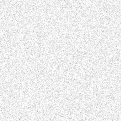
\includegraphics[width=\textwidth]{images/findings/round2/flipbook/loser/checkpoint_000000.png}
	\caption{Starting Weights}
	\end{subfigure}
	~
	\begin{subfigure}[t]{0.2\textwidth}
	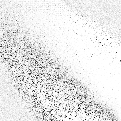
\includegraphics[width=\textwidth]{images/findings/round2/flipbook/loser/checkpoint_200000.png}
	\caption{After 200,000 games played}
	\end{subfigure}
	~
	\begin{subfigure}[t]{0.2\textwidth}
	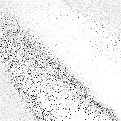
\includegraphics[width=\textwidth]{images/findings/round2/flipbook/loser/checkpoint_400000.png}
	\caption{After 400,000 games played}
	\end{subfigure}

	\begin{subfigure}[t]{0.2\textwidth}
	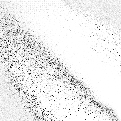
\includegraphics[width=\textwidth]{images/findings/round2/flipbook/loser/checkpoint_600000.png}
	\caption{After 600,000 games played}
	\end{subfigure}
	~
	\begin{subfigure}[t]{0.2\textwidth}
	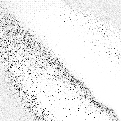
\includegraphics[width=\textwidth]{images/findings/round2/flipbook/loser/checkpoint_800000.png}
	\caption{After 800,000 games played}
	\end{subfigure}
	~
	\begin{subfigure}[t]{0.2\textwidth}
	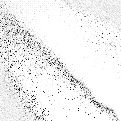
\includegraphics[width=\textwidth]{images/findings/round2/flipbook/loser/checkpoint_999999.png}
	\caption{Final Weights}
	\end{subfigure}

\caption{
	Training weights representation for a losers' bracket agent's \handmaxavg\
	strategy when the agent is the dealer
	over the course of the one million games of Round 2.
}
\label{fig:r2-flip-loser}
\end{figure}


% Figure for the flipbook of strategies over time

\begin{figure}
\center

	\begin{subfigure}[b]{0.4\textwidth}
	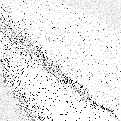
\includegraphics[width=\linewidth]{images/findings/round2/flipbook/winner/checkpoint_000000.png}
	\caption{Starting Weights}
	\end{subfigure}
	~
	\begin{subfigure}[b]{0.4\textwidth}
	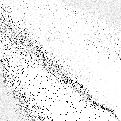
\includegraphics[width=\linewidth]{images/findings/round2/flipbook/winner/checkpoint_200000.png}
	\caption{After 200,000 games played}
	\end{subfigure}

	\begin{subfigure}[b]{0.4\textwidth}
	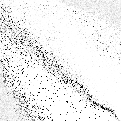
\includegraphics[width=\linewidth]{images/findings/round2/flipbook/winner/checkpoint_400000.png}
	\caption{After 400,000 games played}
	\end{subfigure}
	~
	\begin{subfigure}[b]{0.4\textwidth}
	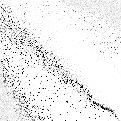
\includegraphics[width=\linewidth]{images/findings/round2/flipbook/winner/checkpoint_600000.png}
	\caption{After 600,000 games played}
	\end{subfigure}

	\begin{subfigure}[b]{0.4\textwidth}
	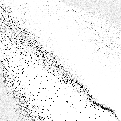
\includegraphics[width=\linewidth]{images/findings/round2/flipbook/winner/checkpoint_800000.png}
	\caption{After 800,000 games played}
	\end{subfigure}
	~
	\begin{subfigure}[b]{0.4\textwidth}
	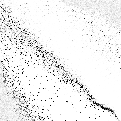
\includegraphics[width=\linewidth]{images/findings/round2/flipbook/winner/checkpoint_999999.png}
	\caption{Final Weights}
	\end{subfigure}

\caption{
	Training weights representation for a winner bracket agent's \handmaxavg\
	strategy when the agent is the dealer
	over the course of the one million games of Round 2.
	Note that the starting weights are carried over from Round 1,
	so the total training epochs to reach each position is actually
	one million higher than expressed.
}
\label{fig:r2-flip-winner}
\end{figure}




%%%
The pairing of a learning agent with a non-learning, randomly weighted agent
provided no additional benefit.
%
The same behavioral trends seen in the losers' bracket are echoed
in Figure~\ref{r2-strats-random}.
%
The lack of clarity found in the images is the result of
fewer games being played because of batch job scheduling issues.
%
From these images,
it becomes clear that the learning mechanism,
as is,
is not conducive to playing a better game of cribbage.
%
Thus there needs to be some form of adjustment made in the framework.
%%%


\begin{figure}
\center

	\begin{subfigure}[t]{0.22\textwidth}
		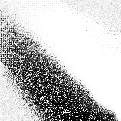
\includegraphics[width=\stratgraphwidth]{images/findings/round2/strats/random/hand_max_min.png}
		\caption{\handmaxmin}
	\end{subfigure}
	~
	\begin{subfigure}[t]{0.22\textwidth}
		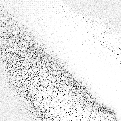
\includegraphics[width=\stratgraphwidth]{images/findings/round2/strats/random/hand_max_avg.png}
		\caption{\handmaxavg}
	\end{subfigure}
	~
	\begin{subfigure}[t]{0.22\textwidth}
		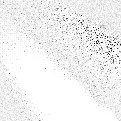
\includegraphics[width=\stratgraphwidth]{images/findings/round2/strats/random/hand_max_med.png}
		\caption{\handmaxmed}
	\end{subfigure}
	~
	\begin{subfigure}[t]{0.22\textwidth}
		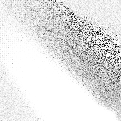
\includegraphics[width=\stratgraphwidth]{images/findings/round2/strats/random/hand_max_poss.png}
		\caption{\handmaxposs}
	\end{subfigure}

	\begin{subfigure}[t]{0.22\textwidth}
		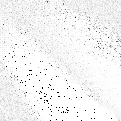
\includegraphics[width=\stratgraphwidth]{images/findings/round2/strats/random/crib_min_avg.png}
		\caption{\cribminavg}
	\end{subfigure}
	~
	\begin{subfigure}[t]{0.22\textwidth}
		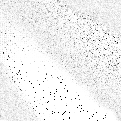
\includegraphics[width=\stratgraphwidth]{images/findings/round2/strats/random/pegging_max_avg_gained.png}
		\caption{\peggingmaxavggained}
	\end{subfigure}
	~
	\begin{subfigure}[t]{0.22\textwidth}
		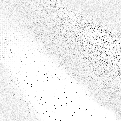
\includegraphics[width=\stratgraphwidth]{images/findings/round2/strats/random/pegging_max_med_gained.png}
		\caption{\peggingmaxmedgained}
	\end{subfigure}
	~
	\begin{subfigure}[t]{0.22\textwidth}
		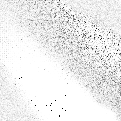
\includegraphics[width=\stratgraphwidth]{images/findings/round2/strats/random/pegging_min_avg_given.png}
		\caption{\peggingminavggiven}
	\end{subfigure}

\caption{
	All final strategy strengths for a learning agent
	after playing a completely random agent
	when playing as the pone
	after training for 350,000 games during Round 2.
}
\label{fig:r2-strats-random}
\end{figure}



%%%
% Section on why the hell nothing seems to work (speculation)
%%%


\paragraph*{Potential Issues}
\label{sec:findings-r2-potentialissues}

%%%
Before modifications can be made to the learning framework,
the comparable performance to random weights must first be addressed as a potential
error in implementation rather than in training.
%
Since all methods of training so far have resulted in very similar policies
being learned,
it is fair to say that policy learned during training has been superior to
random in some manner.
%
There are then a couple items to consider with regard to why such poor results are occurring
during the review tournaments,
such as the scale of play and potential overfitting of the model.
%%%


%%%\subparagraph*{Overfitting}
%%%
%%%%%%
%%%% Overfitting
%%%The first item to consider as the source of the discrepancy between the
%%%observation that a policy is learned,
%%%but its performance is abysmal,
%%%is that the weights table is overfitting to the problem.
%%%%
%%%This would have been especially true of the first round where learning rates
%%%were much higher.
%%%%
%%%However,
%%%if the agents were to be overfitting,
%%%a number of differences would be found in their results.
%%%%
%%%Firstly,
%%%a different set of policy graphs would likely result from the training phase,
%%%which is not the case.
%%%%
%%%More importantly,
%%%a definitive curve would be present in the tournament graphs as performance
%%%would increase before dropping.
%%%%
%%%As can be seen in Figure~\ref{fig:r2-time-series},
%%%this is not the case
%%%as performance is not apparently linked to training in any way.
%%%%
%%%Therefore, it would seem safe to conclude that overfitting is not the reason
%%%for the poor resulting performance.
%%%%%%


\subparagraph*{Scale of Play}

%%%
The prevailing theory as to the reason for which the agent learns a policy,
but following that policy does not yield positive results in performance,
is the issue of scale.
%
The agent is trained on a million games,
but tested on only a handful.
%
Since the cards being dealt are not taken into account by the policy,
the decisions made will likely be inaccurate on the scale of a single game,
but not for thousands.
%%%

% Figures

\begin{figure}
\center
\begin{subfigure}[b]{0.45\textwidth}
	\center
	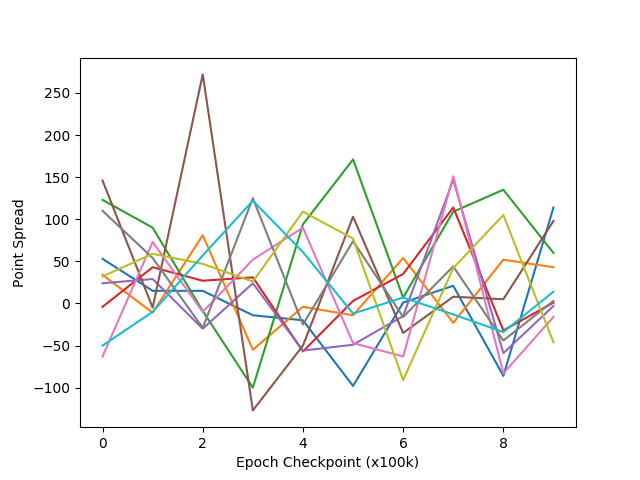
\includegraphics[width=\textwidth]{images/discussion/usefulness/r2-time-series-9.png}
	\caption{Point spreads for 9-game matches} %, like in human play.}
	\label{fig:r2-time-series-9}
\end{subfigure}
~
\begin{subfigure}[b]{0.45\textwidth}
	\center
	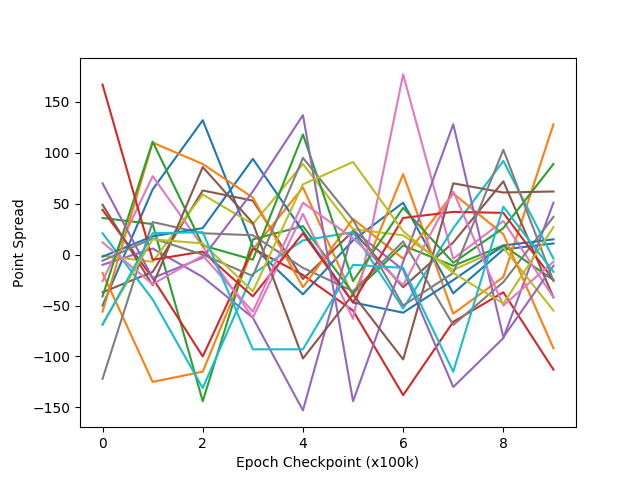
\includegraphics[width=\textwidth]{images/discussion/usefulness/r2-time-series-100.png}
	\caption{Point spreads for 100-game matches.}
	\label{fig:r2-time-series-100}
\end{subfigure}

\begin{subfigure}[b]{0.66\textwidth}
	\center
	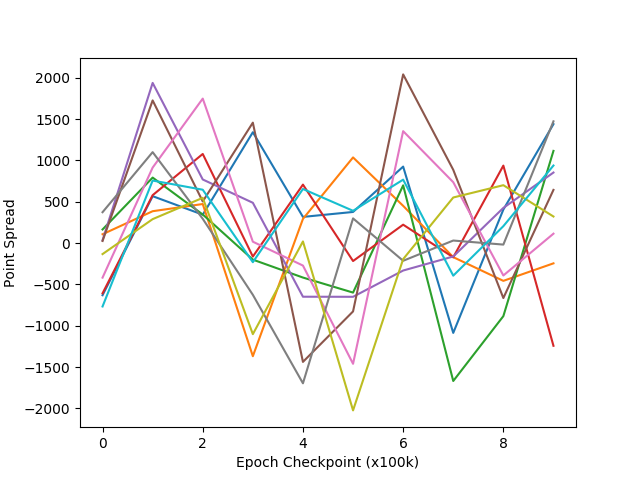
\includegraphics[width=\textwidth]{images/discussion/usefulness/r2-time-series-1000.png}
	\caption{Point spreads for 1,000-game matches.}
	\label{fig:r2-time-series-1000}
\end{subfigure}

\begin{subfigure}[b]{0.66\textwidth}
	\center
	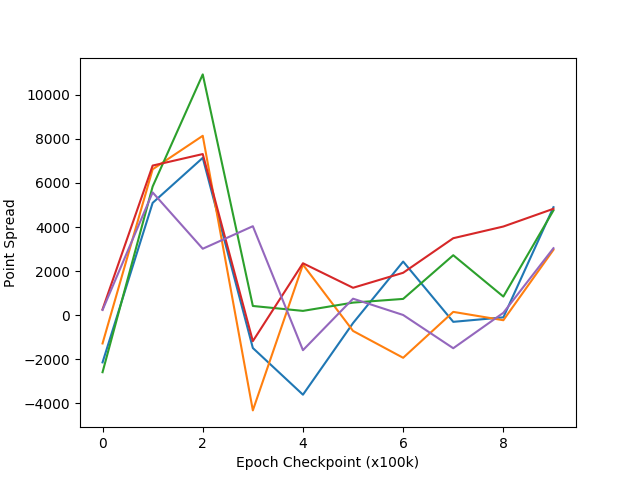
\includegraphics[width=\textwidth]{images/discussion/usefulness/r2-time-series-10000.png}
	\caption{Point spreads for 10,000-game matches.}
	\label{fig:r2-time-series-10000}
\end{subfigure}

\caption{
	Point spreads across matches of varying lengths.
	In each graph,
	the final trained agent is played against its previous checkpoint
	iterations.
}
\label{fig:r2-time-series}
\end{figure}

% /Figures

%%%
% Discussion of how scale affects score spreads
%	On 9-game scale, we have utter chaos, maybe not worth mentioning?
%	On 100-game scale, utter chaos
%	On 1000-game scale, maybe a little, if we squint hard,
%	On 10k-game scale, we can see a pattern
%		contradicts the 1k-game observations
%		consistently even with random
%		sharp increase in performance over 100k-200k
%		even play for the next 600k
%		seemingly regain advantage in the last 200k
%%%

%%%
A regulation cribbage match between two human players consists of nine games.
%
As can be seen in Figure~\ref{fig:r2-time-series-100},
in a series of 100-game matches between a fully trained agent and its
previous checkpoints\textemdash
using a Round 2-trained agent in the losers' bracket for demonstrative
purposes\textemdash
no pattern is discernible in total point spreads between the two playing agents.
%
This demonstrates that,
on this scale,
the winner of the game is no more predictable than a truly random coin toss.
%%%

%%%
When the scale is increased to one thousand games,
a slight pattern begins to emerge
when visualized in Figure~\ref{fig:r2-time-series-1000}.
%
Whereas the majority of the graph remains highly varying and unpatterned,
the first few games begin to trace a common curve.
%
The match against the random agent is still unpredictable,
but the matches against the 100,000 and 200,000 game trained checkpoints are
consistently beaten by the final agent.
%%%

%%%
Although fewer matches are played to compensate for the additional time needed to
play the increased number of games,
the same pattern beginning to form in the thousand-game scale is visible in the
ten thousand-game matches.
%
With the exception of the purely untrained agent,
the least \learned\ agents perform the poorest against the final
\learned\ agent.
%
Play is approximately evenly matched between the fully trained agent
and its checkpoints which have been trained for 300,000 to 700,000 games.
%
Following these matches,
the agent begins to, again, win more consistently when more training is done.
%
This confusingly indicates that more recent agents are getting worse
than earlier iterations,
yet the final agent is better than these.
%
The reasons for this trend are unknown.
%%%

\subparagraph*{Overfitting}

%%%
If the agent is being trained correctly and no overfitting is occurring,
then the point spread should be a positive number,
gradually decreasing and approaching zero
as more training is applied to its opponent,
forming a similar curve to a loss metric used in classical machine learning.
%
In the event of overfitting,
the curve would dip below the zero before reapproaching zero.
%
Neither of these shapes were seen in the resulting graph
(Figure~\ref{fig:r2-time-series-10000}).
%
Instead,
the shape of the curve implies that,
since the random agent performs consistently better than the trained agent,
the learning process is not learning the game so much as how to outplay
or edge out its
opponent in some experienced scenarios that do not
generalize to the testing phase.
%reappear during testing.
%
This conclusion is supported by the observation that the agents with limited
training are steadfastly outplayed.
%%%

%%%
Also of further note, is the scale on the aforementioned graphs.
%
In Figure~\ref{fig:r2-time-series-10000},
the maximum point spread achieved is just a shade above 10,000 points
over the course of 10,000 games.
%
This means that the average point spread advantage is approximately 
one point per game at peak performance\textemdash
and most often $0.2$ points per game\textemdash
in long-term play.
%
The average spread increases to about $30$ points per game when fewer games are 
played,
but since performance is unpredictable on this scale,
this can be explained as a result of the randomness of the cards given
and cannot be considered a reliable measure of performance.
%%%%
%%%In fact,
%%%in sampled matches,
%%%it was not uncommon to observe losses and wins of 30 points or more
%%%as well as much closer games with margins of only a few points.
%
In addition to the randomness of cards dealt,
this massive point sway could also be the result of the agents' uncertainty on 
how to recover from a losing position.
%
While the reasons for this inability cannot be said to be more than speculation,
the learning of a policy directly, without taking into account cards dealt,
is the likely culprit,
as explained previously.
%%%



